%%%%%%%%%%%%%%%%%%%%%%%%%%%%%%%%%%%%%%%%%
% University/School Laboratory Report
% LaTeX Template
% Version 3.1 (25/3/14)
%
% This template has been downloaded from:
% http://www.LaTeXTemplates.com
%
% Original author:
% Linux and Unix Users Group at Virginia Tech Wiki 
% (https://vtluug.org/wiki/Example_LaTeX_chem_lab_report)
%
% License:
% CC BY-NC-SA 3.0 (http://creativecommons.org/licenses/by-nc-sa/3.0/)
%
%%%%%%%%%%%%%%%%%%%%%%%%%%%%%%%%%%%%%%%%%

%----------------------------------------------------------------------------------------
%	PACKAGES AND DOCUMENT CONFIGURATIONS
%----------------------------------------------------------------------------------------

\documentclass{article}

\usepackage{polski}
\usepackage[utf8]{inputenc}
\usepackage{booktabs}
\usepackage{multirow}
\usepackage{caption}
\usepackage{pbox}

\usepackage[version=3]{mhchem} % Package for chemical equation typesetting
\usepackage{siunitx} % Provides the \SI{}{} and \si{} command for typesetting SI units
\usepackage{graphicx} % Required for the inclusion of images
\usepackage{natbib} % Required to change bibliography style to APA
\usepackage{amsmath} % Required for some math elements 

\setlength\parindent{0pt} % Removes all indentation from paragraphs

\renewcommand{\labelenumi}{\alph{enumi}.} % Make numbering in the enumerate environment by letter rather than number (e.g. section 6)

%\usepackage{times} % Uncomment to use the Times New Roman font

%----------------------------------------------------------------------------------------
%	DOCUMENT INFORMATION
%----------------------------------------------------------------------------------------

\title{Ćwiczenie nr 82: Efekt fotoelektryczny} % Title

\author{Rafał \textsc{Grabiański} i Zbigniew \textsc{Królikowski}} % Author name

\date{\today} % Date for the report

\addtolength{\oddsidemargin}{-.875in}
\addtolength{\evensidemargin}{-.875in}
\addtolength{\textwidth}{1.75in}
\addtolength{\topmargin}{-.875in}
\addtolength{\textheight}{1.75in}

\begin{document}

% Please add the following required packages to your document preamble:
% \usepackage{booktabs}
\begin{table}[h]
\begin{tabular}{@{}llllll@{}}
\toprule
\begin{tabular}[c]{@{}l@{}}Wydział:\\ \\ WIEiT\end{tabular}                                    & \multicolumn{2}{l}{\begin{tabular}[c]{@{}l@{}}Imię i nazwisko:\\ Rafał Grabiański\\ Zbigniew Królikowski\end{tabular}}                & \begin{tabular}[c]{@{}l@{}}Rok:\\ \\ II\end{tabular}            & \begin{tabular}[c]{@{}l@{}}Grupa:\\ \\ 7\end{tabular}              & \begin{tabular}[c]{@{}l@{}}Zespół:\\ \\ 7\end{tabular} \\ \midrule
\multicolumn{1}{|c|}{\begin{tabular}[c]{@{}c@{}}PRACOWNIA\\ FIZYCZNA\\ WFiIS AGH\end{tabular}} & \multicolumn{4}{l|}{Temat: Moduł Younga}                                                                                                                                                                                                                                                  & \multicolumn{1}{l|}{Nr ćwiczenia: 11}                     \\ \midrule
\begin{tabular}[c]{@{}l@{}}Data wykonania:\\ \\ \\ 4.11.2014\end{tabular}                     & \begin{tabular}[c]{@{}l@{}}Data oddania:\\ \\ \\ 18.11.2014\end{tabular} & \begin{tabular}[c]{@{}l@{}}Zwrot do poprawy:\\ \\ \\ .\end{tabular} & \begin{tabular}[c]{@{}l@{}}Data oddania:\\ \\ \\ .\end{tabular} & \begin{tabular}[c]{@{}l@{}}Data zaliczenia:\\ \\ \\ .\end{tabular} & OCENA:                                                  \\ \bottomrule
\end{tabular}
\end{table}

%\maketitle % Insert the title, author and date


%----------------------------------------------------------------------------------------
%	SECTION 1 - CEL ĆWICZENIA
%----------------------------------------------------------------------------------------

\section{Cel ćwiczenia}

Celem ćwiczenia było obliczenie modułu Younga dla dwóch drutów metalowych pod obciążeniem stałej siły.

% If you have more than one objective, uncomment the below:
%\begin{description}
%\item[First Objective] \hfill \\
%Objective 1 text
%\item[Second Objective] \hfill \\
%Objective 2 text
%\end{description}


%\clearpage

%----------------------------------------------------------------------------------------
%	SECTION 4
%----------------------------------------------------------------------------------------
\section{Wyniki pomiarów}

\subsection{Dane dotyczące drutów}
\begin{table}[h]
\centering
\begin{tabular}{|l|c|l|c|}
\hline
Rodzaj materiału          & \multicolumn{3}{c|}{stal}                                                                                                                                                                                         \\ \hline
Długość drutu l {[}mm{]}  & 1070                                                           & u(l) {[}mm{]}                                                                    & 1                                                             \\ \hline
Średnica drutu d {[}mm{]} & \begin{tabular}[c]{@{}c@{}}Pomiar pierwszy\\ 0.75\end{tabular} & \multicolumn{1}{c|}{\begin{tabular}[c]{@{}c@{}}Pomiar drugi\\ 0.77\end{tabular}} & \begin{tabular}[c]{@{}c@{}}Pomiar trzeci:\\ 0.78\end{tabular} \\ \hline
Średnica średnia {[}mm{]} & 0.77                                                           & u(d) {[}mm{]}                                                                    & 0.008                                                         \\ \hline
\end{tabular}
\caption{Drut stalowy}
\end{table}

\begin{table}[h]
\centering
\begin{tabular}{|l|c|l|c|}
\hline
Rodzaj materiału          & \multicolumn{3}{c|}{stal}                                                                                                                                                                                         \\ \hline
Długość drutu l {[}mm{]}  & 1070                                                           & u(l) {[}mm{]}                                                                    & 1                                                             \\ \hline
Średnica drutu d {[}mm{]} & \begin{tabular}[c]{@{}c@{}}Pomiar pierwszy\\ 1.15\end{tabular} & \multicolumn{1}{c|}{\begin{tabular}[c]{@{}c@{}}Pomiar drugi\\ 1.14\end{tabular}} & \begin{tabular}[c]{@{}c@{}}Pomiar trzeci:\\ 1.15\end{tabular} \\ \hline
Średnica średnia {[}mm{]} & 1.15                                                           & u(d) {[}mm{]}                                                                    & 0.008                                                         \\ \hline
\end{tabular}
\caption{Drut mosiężny}
\end{table}

\clearpage

\begin{table}[htbp]
\begin{tabular}{|c|c|c|c|c|c|}
\hline
\multicolumn{1}{|l|}{Masa [kg]} & \multicolumn{1}{l|}{Sila [N]} & \{Wskazanie czujnika 1 [mm] & \multicolumn{1}{l|}{Wskazanie czujnika 2 [mm]} & \multicolumn{1}{l|}{Wydłużenie średnie [mm]} \\ \hline

1 & 9.81 & 0.4 & 0.42 & 0.205 \\ \hline
2 & 19.62 & 0.7 & 0.74 & 0.36 \\ \hline
3 & 29.43 & 0.99 & 0.99 & 0.495 \\ \hline
4 & 39.24 & 1.23 & 1.24 & 0.6175 \\ \hline
5 & 49.05 & 1.48 & 1.49 & 0.7425 \\ \hline
6 & 58.86 & 1.71 & 1.72 & 0.8575 \\ \hline
7 & 68.67 & 1.95 & 1.95 & 0.975 \\ \hline
8 & 78.48 & 2.16 & 2.16 & 1.08 \\ \hline
9 & 88.29 & 2.39 & 2.39 & 1.195 \\ \hline
\end{tabular}
\label{}
\caption{Wyniki pomiaru wydłużenia dla drutu stalowego}
\end{table}

\begin{table}[htbp]
\centering
\begin{tabular}{|c|c|c|c|c|}
\hline
\multicolumn{1}{|l|}{Masa [kg]} & \multicolumn{1}{l|}{Siła [N]} & \multicolumn{1}{l|}{Wskazanie czujnika 1 [mm]} & \multicolumn{1}{l|}{Wskazanie czujnika 2 [mm]} & \multicolumn{1}{l|}{Wydłużenie średnie [mm]} \\ \hline
1 & 9.81 & 0.35 & 0.36 & 0.1775 \\ \hline
1.5 & 14.715 & 0.51 & 0.52 & 0.2575 \\ \hline
2 & 19.62 & 0.68 & 0.67 & 0.3375 \\ \hline
2.5 & 24.525 & 0.81 & 0.8 & 0.4025 \\ \hline
3 & 29.43 & 0.92 & 0.94 & 0.465 \\ \hline
3.5 & 34.335 & 1.05 & 1.06 & 0.5275 \\ \hline
4 & 39.24 & 1.17 & 1.18 & 0.5875 \\ \hline
5 & 49.05 & 1.4 & 1.42 & 0.705 \\ \hline
6 & 58.86 & 1.63 & 1.63 & 0.815 \\ \hline
\end{tabular}
\label{}
\caption{Wyniki pomiaru wydłużenia dla drutu mosiężnego}
\end{table}



%----------------------------------------------------------------------------------------
%	SECTION 5 - WYNIKI
%----------------------------------------------------------------------------------------

\section{Opracowanie wyników}
\subsection{Średnice drutów}
Dokonaliśmy pomiaru średnicy drutu za pomocą śruby mikrometrycznej. Wyciągnęliśmy średnią arytmetyczną z trzech pomiarów wykonanych w różnych miejscach dla obo drutów. Niepewność oceniona na podstawie rozdzielczości przyrządu wynosi 1 $\mu m$. Wyniki umieszczono w tabelach 1 i 2.
Niepewność pomiaru grubości oszacowaliśmy na 8$\nu m$. Taka była różnica między zacieśnieniem do oporu śruby mikrometrycznej na drucie, a lekkim dociśnięciem.
\subsection{Obliczenie wartości siły rozciągającej}
Obliczenie siły rozciągającej sprowadzało się do wymnożenia przyspieszenia ziemskiego przez masę obciążającą:

\begin{equation}
	F = m \cdot g
\end{equation}

Za g przyjęliśmy przybliżoną wartość $9.81 \frac{m}{s^{2}}$

\subsection{Obliczenie średniej wartości wydłużenia}
Liczymy średnią arytmetyczną z dwóch pomiarów dokonanych dla każdego obciążenia. Wynik musimy podzielić przez 2 by uwzględnić działanie dźwigni (zmiana wg czujnika jest dwa razy większa od rzeczywistej). Wyniki znajdują się w kolumnach \emph{Wydłużenie średnie} w tabelach 1 i 2.
\clearpage
\subsection{Zależność średniego wydłużenia drutu od przyłożonej siły}

\begin{figure}[h!]
	\centering
	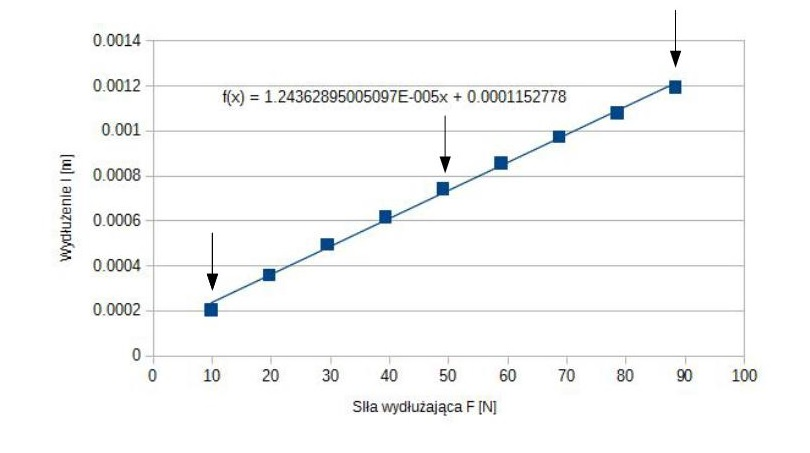
\includegraphics[scale=0.47]{ch01}
	\caption{Wykres zależności wydłużenia drutu stalowego od przyłożonej siły wydłużającej}
\end{figure}

\begin{figure}[h!]
	\centering
	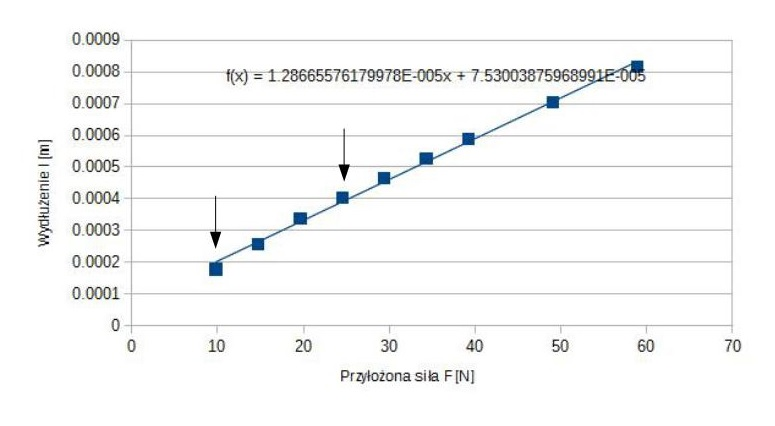
\includegraphics[scale=0.47]{ch02}
	\caption{Wykres zależności wydłużenia drutu mosiężnego od przyłożonej siły wydłużającej}
\end{figure}

\subsection{Dopasowanie prostej do punktów}
Korzystając z programu komputerowego, dopasowaliśmy dla obu drutów prostą aproksymującą je. Nie odrzucliśmy w żadnym przypadku żadnego punktu, gdyż w naszej opinii żaden nie odbiega na tyle by mógł być uznany za błąd gruby w pomiarze.

Ptrzymujemy takie współczynniki prostych:
\begin{itemize}
	\item Drut stalowy: $a = 1.24 \cdot 10^{-5}$, $u(a) = 2.4 \cdot 10^{-7}$
	\item Drut mosiężny: $a = 1.29 \cdot 10^{-5}$, $u(a) = 3.17 \cdot 10^{-7}$
\end{itemize}

\subsection{Wyznaczenie modułu Younga}
Korzystając z przekształceń wykonanych w skrypcie, mamy do dyspozycji wzór roboczy na moduł Younga następującej postaci:
\begin{equation}
	E = \frac{4l}{\pi d^{2} a}
\end{equation}

Zatem moduł Younga przyjmuje wartości:
\begin{itemize}
	\item $E_{stal} = 186.38 $ GPa
	\item $E_{mosi} = 80.51 $ GPa
\end{itemize}

\subsection{Wyznaczenie niepewności}
Korzystając z również wyprowadzonego we wstępie teoretycznym wzoru na niepewność złożoną dla modułu Younga:

\begin{equation}
	\frac{U_{c}(E)}{E} = \sqrt{(\frac{u(l)}{l})^{2}+(-2\frac{u(d)}{d})^{2}+(-\frac{u(a)}{a})^{2}}
\end{equation}

Dla drutu stalowego $\frac{u_{cSTAL}(E)}{E} = 0.03$, natomiast dla wykonanego z mosiądzu: $\frac{u_{cMOSI}(E)}{E} = 0.03$

\subsection{Porównanie wyniku pomiaru do wartości tablicowych}
Przyjmując współczynnik rozszerzenia k = 2 otrzymujemy, że wynik dla stali powinien zawierać się w przedziale [197.4, 233.2]. Uzyskany przez nas wynik 186.4 GPa jest poza tym przedziałem. Powodem tego może być wysłużenie tego drutu, o czym więcej we wnioskach.
Dla mosiądzu docelowy przedział wg tablic to [94, 106], a uzyskano wynik 80.5 GPa, co również nie jest najlepszym przybliżeniem.
%----------------------------------------------------------------------------------------
%	SECTION 6
%----------------------------------------------------------------------------------------
\section{Wnioski}
Wartość dla mosiądzu to 80.5 GPa a tabelaryczna ok. 100 GPa.

Wartość dla stali, 186.4 GPa, podczas gdy tabelaryczna 200-210 GPa.

Otrzymane przez nas wartości odbiegają od tabelarycznych ponad otrzymaną przez nas niepewność. Dopiero dla k=4 nasze wyniki mieszczą blisko wzorcowych. Warto jednak zaznaczyć, że materiał, z którego wykonane są nasze druty nie został dokładnie zidentyfikowany a także ich właściwości mogły ulec zmianie na skutek zużycia(mechaniczego lub czynników środowiskowych np. korozji). Wobec tego rozszerzanie niepewności miałoby sens tylko w przypadku nowych fabrycznie, lub minimalnie zużytych drutów, z modułem Younga jednoznacznie określonym przez producenta.

Interpretacja wyników zależy od tego jak traktujemy wartości tabelaryczne. Doświadczenie było wykonane prawidłowo, procedury proste i trudne do omylenia także otrzymane przez nas wartości traktujemy jako prawidłowe.

%----------------------------------------------------------------------------------------
%	BIBLIOGRAPHY
%----------------------------------------------------------------------------------------

\bibliographystyle{apalike}

\bibliography{sample}
%----------------------------------------------------------------------------------------


\end{document}
